\chapter{Contribution 1 Title}
\chaptermark{Chapter Title for Contents \& Running Page Head}
% Reset the glossary count so acronyms are written in full on first use in the abstract
\glsresetall
\label{chap:3-contribution_1}

\begin{cabstract}
The abstract for this chapter of the Thesis.

Can contain multiple paragraphs.

\blindtext
\end{cabstract}

A small description or statement about the chapter, \eg ``This chapter was published at the SUPER conference in 2020'' \parencite{robinson2020thesis}. 

\section{Overview}
\label{sec:2-overview}
% Reset the glossary count so acronyms are written in full on first use in this chapter (after the abstract)
\glsresetall

An overarching overview of the Chapter contents.

If using this template, you should also attribute the formatting to Rob Robinson \parencite{robinson2020thesis} and link to the original template or thesis \url{https://github.com/mlnotebook}. % overview
\section{Introduction}
\label{sec:3-introduction}

General introduction to the area with which this chapter is concerned. It should set the scene and identify the need for research in this area.

The next chapter deals with the related work which tries to address this need (and places the Thesis research in context).

\subsection{Contributions}

A short introduction to the contributions that are made by the work in this Thesis. % introduction
\section{Related Works}
\label{sec:3-literature}

This section identifies and describes the relevant literature that aims to address the issue raised in the introduction.

\subsection{Some theme around the research area.}

Subsections can be used if the area can be broken down into different strategies or methods for tackling the same problem. Pros/cons of the methods can be addressed and related to how the method presented in the Thesis may overcome these.
 % related works
\section{Materials and Methods}
\label{sec:3-methods}

A short overview of the data and methods that will be introduced in the following subsections - tables, sources \etc

\subsubsection{Some Dataset.}
\label{sec:3-dataset}

Descriptions and examples of the dataset that is being used.
\subsection{Method}
\label{sec:3-method}

This subsection describes the methods used in this Chapter.

Use `fref` to refer to figures as "figure (X.X) on page (X)". `Fref` (note the capital F) will capitalize `figure` to `Figure`. \eg \fref{fig:3-example_figure} or \Fref{fig:3-example_figure}.

\begin{figure}[t]
    \centering
	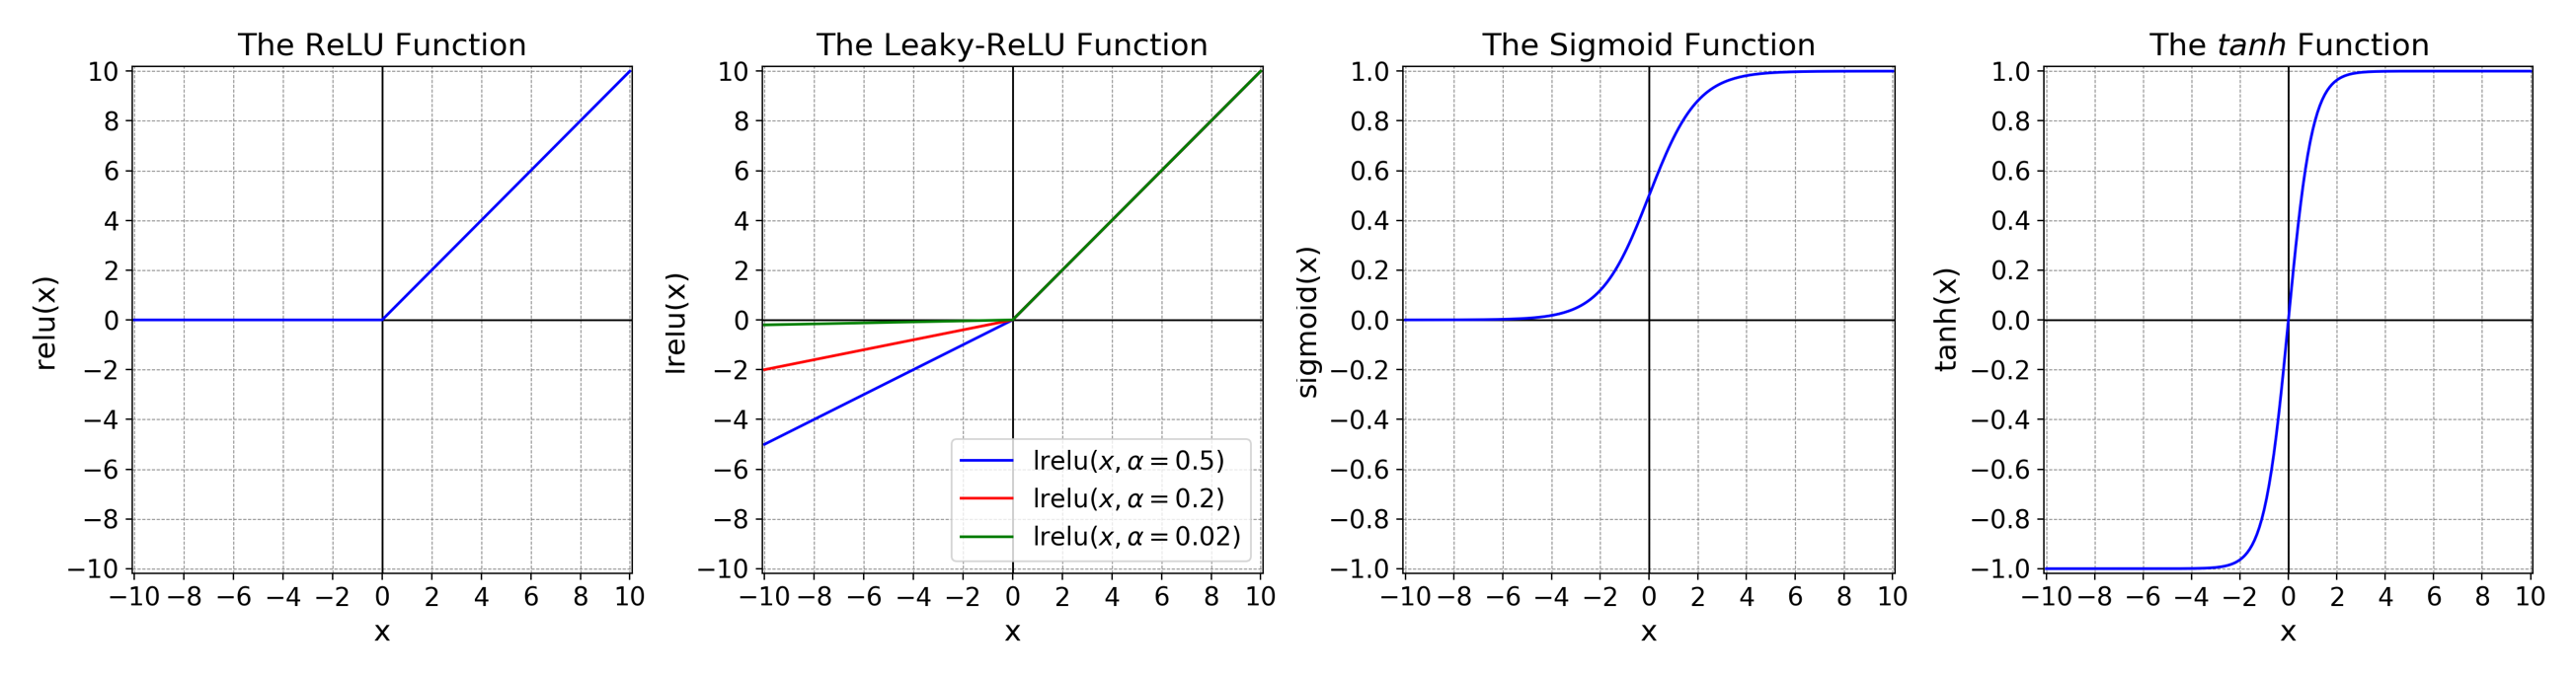
\includegraphics[width=\linewidth]{chapters/chapter3-contribution_1/3-images/example_image.png}
	\mycaption{This is the title of the figure - it will also appear in the contents table.}{This is the rest of the caption. \label{fig:3-example_figure}}
\end{figure}
\subsection{Evaluation Strategies}
\label{sec:3-seg_eval}

This section can hold the methods used for evaluating the experiments performed in the this Chapter.

\subsubsection{Some Metric}

Equations can be used in a number of ways. The \gls{dsc} is used as an example below.

\begin{enumerate}[label=\textbf{\arabic*}]
\item Simple Display Equation: 
% This '%' is necessary to reduce the gap between the text and equation - but it can be useful to keep it if equations spill over pages (thus the skip has not been hardcoded)
\begin{equation}
    \mathrm{DSC} = \frac{2 \left|\textbf{A} \cap \textbf{B}\right|}{\left|\textbf{A}\right| + \left|\textbf{B}\right|} \label{eq:simple_display_equation}   
\end{equation}

\item Annotated Display Equation: `falign` adds a title to the left (or right) of the equation. Uses the table cell notation `\&\&` to separate the left, middle and right parts.
% 
\begin{flalign}
    \text{Dice Similarity Coefficient:\quad} &&\mathrm{DSC} = \frac{2 \left|\textbf{A} \cap \textbf{B}\right|}{\left|\textbf{A}\right| + \left|\textbf{B}\right|} \label{eq:dsc}&&    
\end{flalign}

\item Multi-Equation: `align` can align multiple equations by using the `\&` symbol on the equals sign and `\textbackslash\textbackslash` where the newline begins. Multiple labels can be used - one for each equation.
% 
\begin{align}
    y &= (x+1)^2 \label{eq:aligned_1}\\
    y &= (x^2 + 2x + 1) \label{eq:aligned_2}
\end{align}

\end{enumerate}




 % methods
\section{Results}
\label{sec:3-results}

An introduction to the results.

\subsection{Experiment A Results: Experiment name.}
\label{sec:3-exp_a_results}

Tables are enclosed in a 'colorbox' which makes the background white against the 'mdframe' of the float object. Checks and crosses are created from custom commands that use dings: \texttt{\textbackslash cmark} and \texttt{\textbackslash xmark}.

\begin{table}[h!]
  \mycaption{Caption Title goes here (appears in TOC).}{Rest of the caption goes here \label{tab:example_table}}
  \centering
  \colorbox{white}{
      \begin{tabular}{ccccc}
      \hline 
      \textbf{Experiment}  		& \textbf{Dataset} 				& \textbf{Size} 		& \textbf{GT} 		& \textbf{Seg. Method} 	\\	\hline		
      A 		& Hammersmith   & 100		& \cmark		& RF 			\\
      B 		& UKBB-2964	    & 4,805		& \cmark		& RF and CNN  	\\
      C 		& UKBB-18545	& 7,250		& \xmark		& Multi-Atlas	\\   \hline
      \end{tabular}
  }%colorbox
\end{table}


Multiple tables can be stacked using minipages. Note the \texttt{[t]} in the minipages to keep them aligned at the top.

\begin{table}[h]
    \centering
    \mycaption{Table Title (appears in TOC)}{The rest of the caption goes here. \label{tab:3-example_results}}
    \colorbox{white}{
    \begin{minipage}[t]{0.5\linewidth}
        \begin{tabular}[t]{r | c c c c}
            \textbf{Class}	&   \textbf{Metric}  &    \textbf{Acc}.	&	\textbf{TPR}	&	\textbf{FPR}	\\
            \hline							
            \textbf{LVC}	&	DSC	&	0.998	&	1.000	&	0.000	\\
            	&	MSD	&	1.000	&	1.000	&	0.000	\\
            \textbf{LVM}	&	DSC	&	0.051	&	1.000	&	0.001	\\
            	&	MSD	&	1.000	&	1.000	&	0.000	\\
            \textbf{RVC}	&	DSC	&	0.901	&	1.000	&	0.033	\\
            	&	MSD	&	0.997	&	0.997	&	0.000	\\
            \textbf{Av.}	&	DSC	&	0.650	&	1.000	&	0.011	\\
            	&	MSD	&	0.999	&	0.999	&	0.000	\\
            \textbf{WH}	&	DSC	&	\textbf{0.998}	& \textbf{1.000}	&	\textbf{0.000}	\\
            	&	MSD	&	\textbf{1.000}	&	\textbf{1.000}	&	\textbf{0.000}	\\
        \end{tabular}
    \end{minipage}
    \hfill
    \begin{minipage}[t]{0.45\linewidth}
        \begin{tabular}[t]{r | c c c c}
            & \multicolumn{4}{c}{\textbf{MAE}} \\
            \hline
            \thead{\textbf{Class}} & \thead{\textbf{DSC}\\} & \thead{\shortstack{\textbf{MSD}\\(mm)}} & \thead{\shortstack{\textbf{RMS}\\(mm)}} & \thead{\shortstack{\textbf{HD}\\(mm)}}\\
            \hline									
            \textbf{LVC}	&	0.082	&	0.386	&	0.442	&	1.344	\\
            \textbf{LVM}	&	0.268	&	0.510	&	0.547	&	2.127	\\
            \textbf{RVC}	&	0.146	&	0.588	&	0.656	&	2.086	\\
            \textbf{Av.}	&	0.165	&	0.495	&	0.548	&	1.852	\\
            \textbf{WH}	&	\textbf{0.089}	&	\textbf{0.460}	&	\textbf{0.509}	&	\textbf{1.698}	\\
        \end{tabular}
    \end{minipage}
    }%colorbox
\end{table}

 % results
\section{Conclusions}
\label{sec:3-conclusions}

A list of the conclusions from the chapter. Each with a title and an explanation.

\begin{enumerate}[wide, labelindent=0pt, label=\textbf{\Alph*}]

%%%%%%%%%%%%%%%%%%%%%%%%%%%%%%%%%%%%%%%%%%%%%%
\item\textbf{Conclusion 1 Title}

Explanation of Conclusion 1.

%%%%%%%%%%%%%%%%%%%%%%%%%%%%%%%%%%%%%%%%%%%%%%
\item\textbf{Conclusion 2 Title}

Explanation of Conclusion 2.

\end{enumerate} % conclusions

